\documentclass[tikz,border=10pt]{standalone}
\usepackage{amsmath} % 用于显示分数
\usepackage{amssymb}
\usetikzlibrary{angles,quotes,backgrounds}

\begin{document}
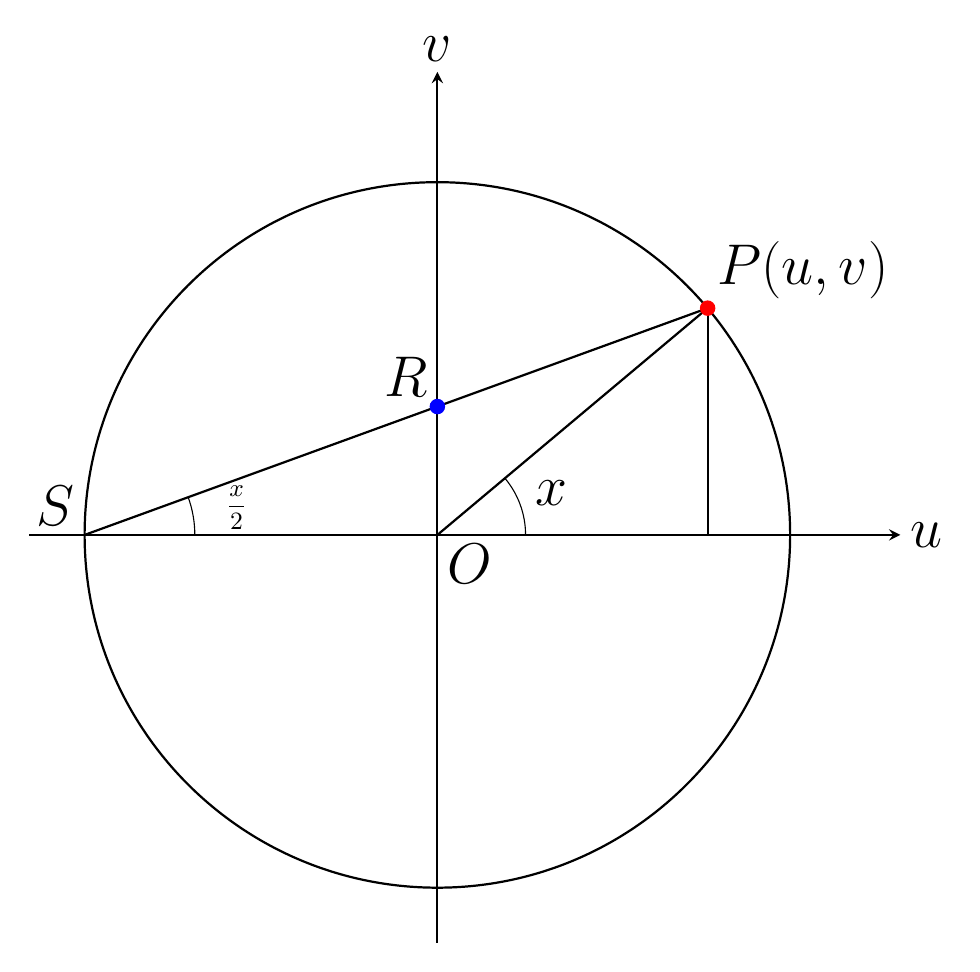
\begin{tikzpicture}[>=stealth, scale=1.4]

% --- 全局设置更大的标签字体 ---
\tikzset{every node/.style={font=\huge}}

% --- 设置参数 ---
\def\circRadius{3.2}   % 圆的半径
\def\angleX{40}        % O点的角度 x (度数)
\def\angleXhalf{20}    % S点的角度 x/2 (近似，基于定理)

% --- 定义关键点 ---
\coordinate (O) at (0, 0);
\coordinate (S) at (-\circRadius, 0);
\coordinate (P) at (\angleX:\circRadius);
\coordinate (Px) at ({\circRadius*cos(\angleX)}, 0); % P在u轴上的垂足
\coordinate (R) at (0, {\circRadius*tan(\angleXhalf)}); % R是SP与v轴的交点

% --- 绘制圆 ---
\draw[thick] (O) circle (\circRadius);

% --- 绘制坐标轴 (u, v) ---
\draw[->, thick] (-\circRadius-0.5, 0) -- (\circRadius+1, 0) node[right, font=\huge] {$u$};
\draw[->, thick] (0, -\circRadius-0.5) -- (0, \circRadius+1) node[above, font=\huge] {$v$};

% --- 绘制几何线条 ---
\draw[thick] (S) -- (P);     % 弦 SP
\draw[thick] (O) -- (P);     % 半径 OP
\draw[thick] (Px) -- (P); % P点向u轴的垂线

% --- 绘制点 P 和 R 的实心圆 ---
\fill[red] (P) circle (2pt);
\fill[blue] (R) circle (2pt);

% --- 添加顶点标签 (更大字体) ---
\node[below right] at (O) {$O$};
\node[above left] at (S) {$S$};
\node[above right, font=\huge] at (P) {$P(u,v)$}; % 比其他标签略小，但仍清晰
\node[above left] at (R) {$R$};

% --- 添加角度标记和标签 ---
% 原点 O 处的角度 x
\begin{scope}
    \draw ([shift=(0:0.8)]O) arc (0:\angleX:0.8);
    \node at (20:1.1) {\huge$x$}; % 将 x 放在弧线外部
\end{scope}

% 点 S 处的角度 x/2
\begin{scope}
    \draw ([shift=(0:1.0)]S) arc (0:\angleXhalf:1.0);
    % 关键修改：将分数标签移至弧线外部 (进一步偏移)
    \node at ([shift=(10:1.4)]S) {\small$\dfrac{x}{2}$}; % 使用 \dfrac 强制大显示模式
\end{scope}
\end{tikzpicture}
\end{document}